\question{Câu 1}

Thiết kế mạch thực hiện hàm: $V_{o} = 2V_{1} + 3V_{2} - 6V_{3}$ với yêu cầu chỉ sử dụng 2 OPAMP.

\answer{a}{Giả sử các OPAMP sử dụng là lý tưởng.}

Ta có: $V_{o}= 2V_1 + 3V_2 - 6V_3$

\begin{itemize}[label=-]
	\item Chọn mạch khuếch đại cộng đảo để thiết kế cho tầng 1:
	\[V_{o1} = -2V_{1} - 3V_{2}\]
	Chọn $R_F = 30\,\textsf{k}\Omega \Rightarrow \left\{ \begin{matrix}
		R_{1} = 15\,\textsf{k}\Omega \\[4pt]
		R_{2} = 10\,\textsf{k}\Omega
	\end{matrix} \right.$ 
	
	\begin{figure}[H]
		\centering
		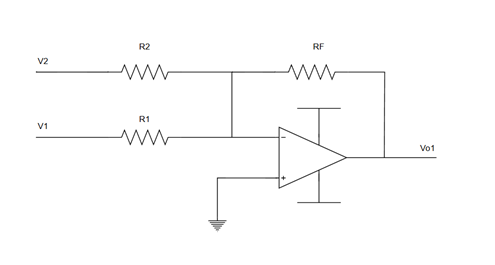
\includegraphics[width=.8\linewidth]{./my-chapters/my-images/Question1/câu 1 a tầng 1.png}
		\caption{Mạch thực hiện $V_{o1} = -2V_{1} - 3V_{2}$.}
	\end{figure}
	
	\item Chọn mạch khuếch đại cộng đảo thiết kế cho tàng 2:
	\[ V_o = -v_{o1} - {6V}_3 \]
	Chọn $R_G = 60\,\textsf{k}\Omega \Rightarrow \left\{ \begin{matrix}
		R_{3} = 10\,\textsf{k}\Omega \\[4pt]
		R_{4} = 60\,\textsf{k}\Omega
	\end{matrix} \right.$ 
	
	\begin{figure}[H]
		\centering
		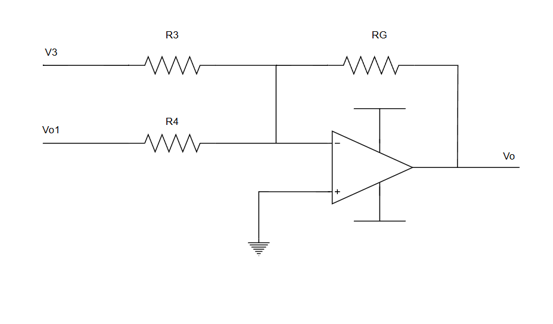
\includegraphics[width=.8\linewidth]{./my-chapters/my-images/Question1/Câu 1 a tầng 2.png}
		\caption{Mạch thực hiện $V_o = -v_{o1} - {6V}_3$.}
	\end{figure}
	
	\item Mạch hoàn chỉnh:
	
	\begin{figure}[H]
		\centering
		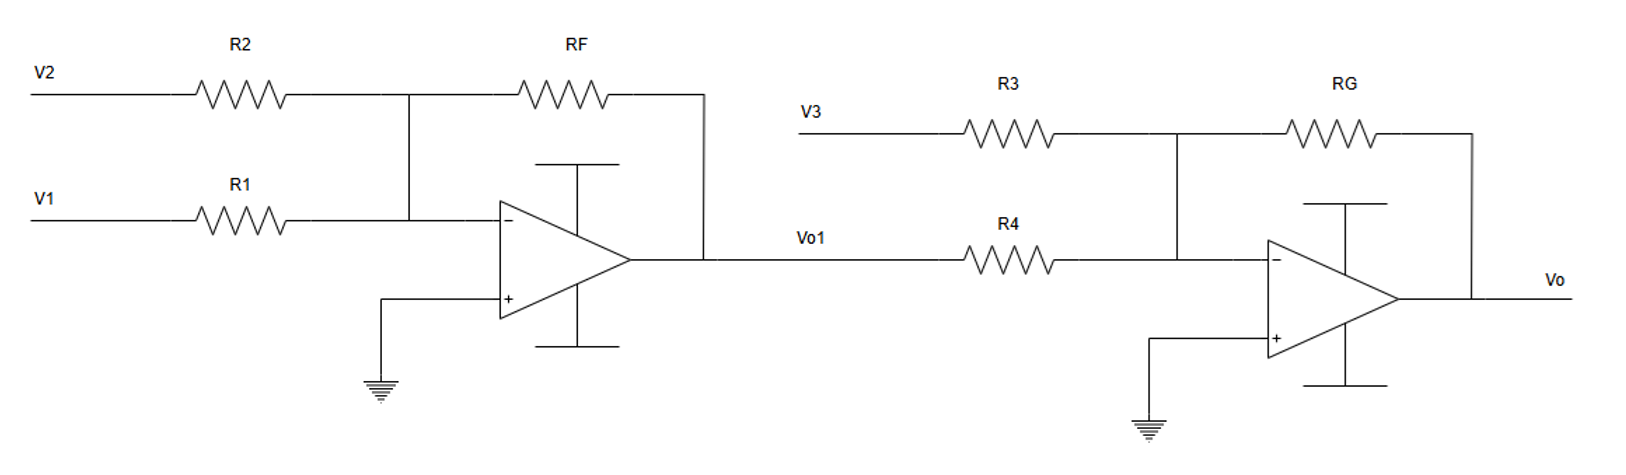
\includegraphics[width=.9\linewidth]{./my-chapters/my-images/Question1/a_mach_hoan_chinh.png}
		\caption{Mạch hoàn chỉnh thực hiện $V_{o} = 2V_{1} + 3V_{2} - 6V_{3}$.}
	\end{figure}
	
	\item Thưc hiện mô phỏng trên Multisim:
	
	\begin{figure}[H]
		\centering
		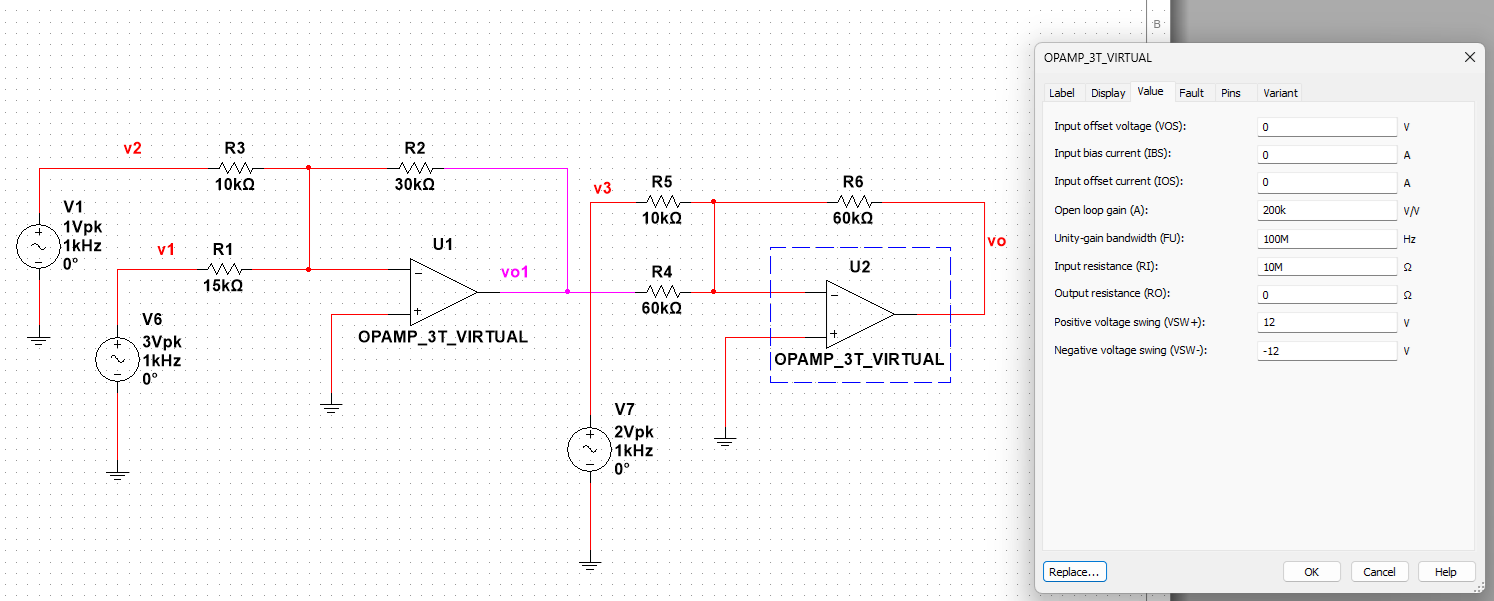
\includegraphics[width=.9\linewidth]{./my-chapters/my-images/Question1/a_mach_mo_phong.png}
		\caption{Thiết kế mạch $V_{o} = 2V_{1} + 3V_{2} - 6V_{3}$ với OPAMP lý tưởng.}
	\end{figure}
	
	\begin{figure}[H]
		\centering
		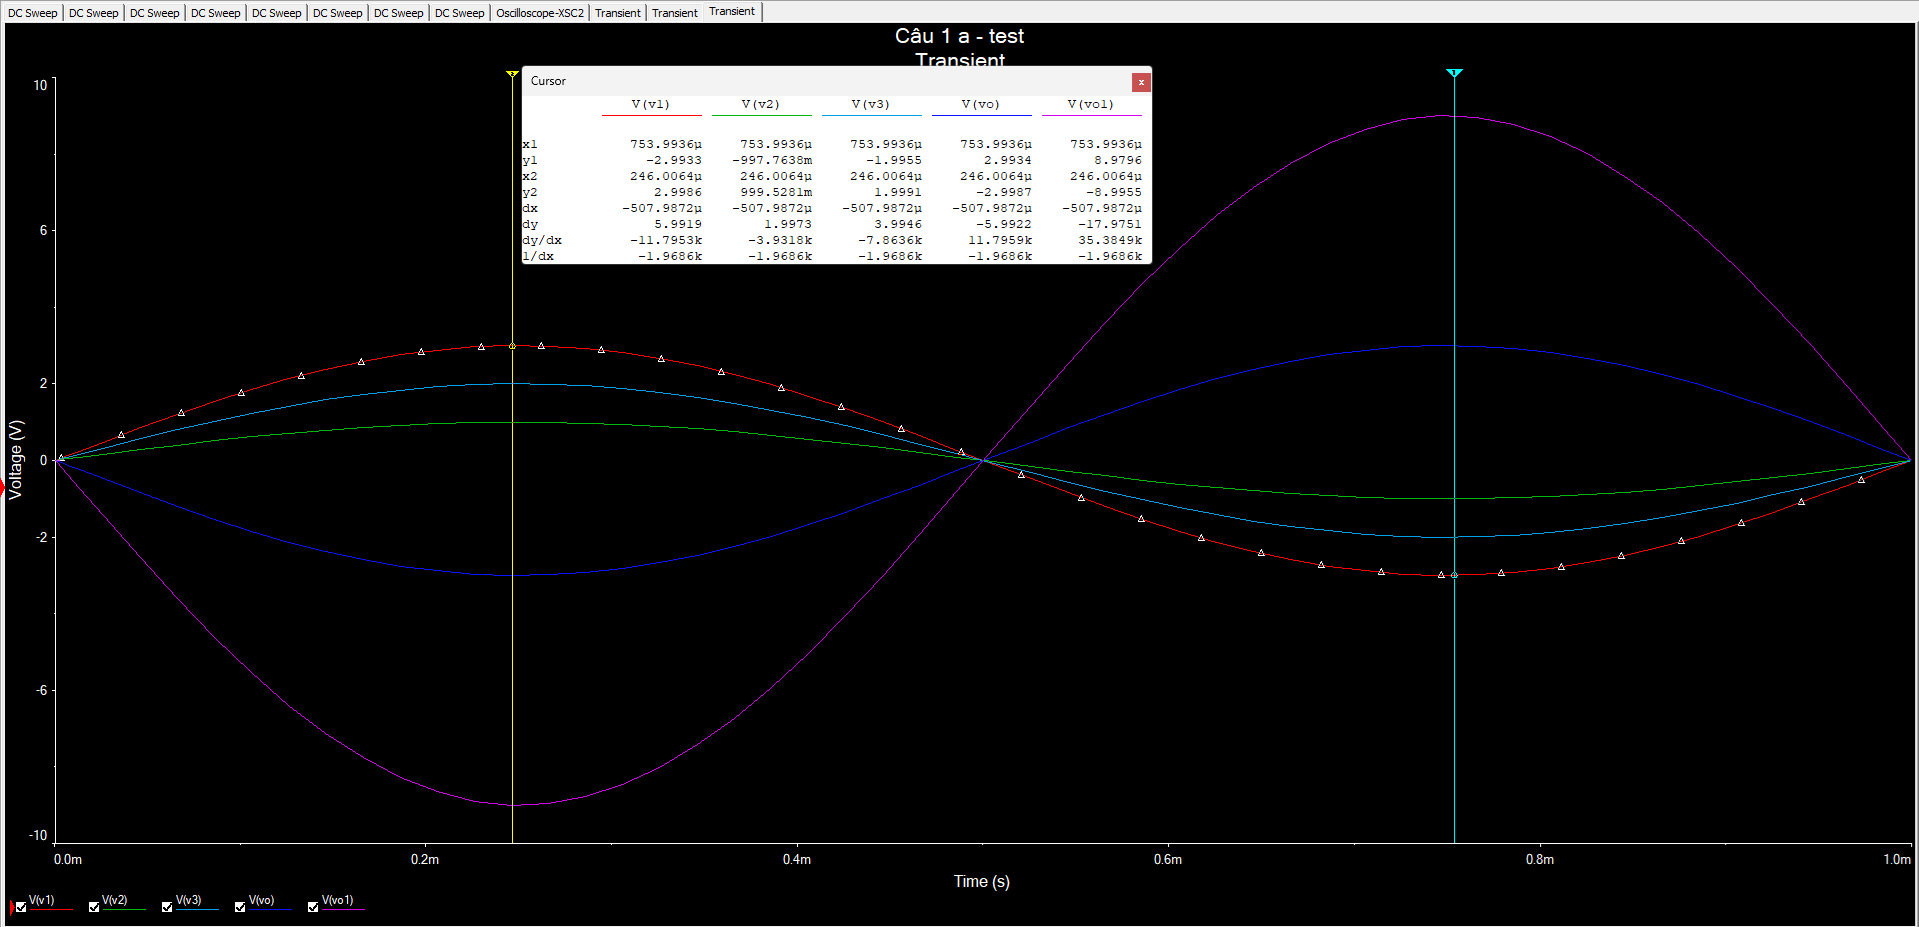
\includegraphics[width=.9\linewidth]{./my-chapters/my-images/Question1/a_ketqua_lytuong.png}
		\caption{Kế quả của mạch $V_{o} = 2V_{1} + 3V_{2} - 6V_{3}$ với OPAMP lý tưởng.}
	\end{figure}
	
	\begin{minipage}{.7\linewidth}
		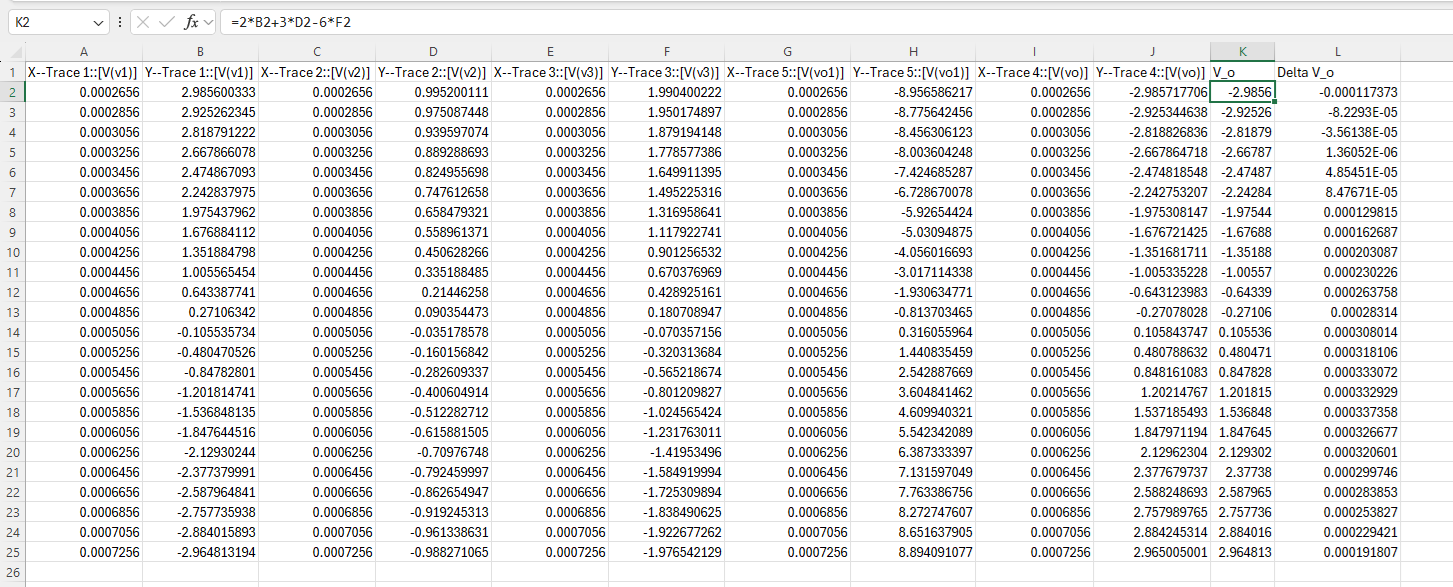
\includegraphics[width=\linewidth]{./my-chapters/my-images/Question1/a_saiso_lytuong.png}
	\end{minipage}
	\begin{minipage}{.3\linewidth}
		\begin{itemize}[label=-]
			\item \finalresult{\Delta V_{o_{max}} = 0.000337358 \,\textsf{V}}
			\item \finalresult{\Delta V_{o_{min}} = -0.000117373 \,\textsf{V}}
		\end{itemize}
	\end{minipage}
	
\end{itemize}

\answer{b}{Giả sử cả 2 OPAMP có $V_{io} = 100\,\mu\textsf{V}$, $I_{io} = 4\,\textsf{nA}$, $I_{ib} = 18\,\textsf{nA}$. Tìm điều kiện ảnh hưởng của điều kiện không lý tưởng của OPAMP lên ngõ ra $V_{o}$.}

\begin{itemize}[label=-]
	\item Xét ảnh hưởng ở tầng 1
		\begin{itemize}[label=+]
			\item Ảnh hưởng do $V_{io}$ gây ra:
			\[ \Delta V_{1} = \left( 1 + \dfrac{R_{F}}{R_{1} // R_{2}} \right) V_{io} = 6V_{io} = 600\,\mu\textsf{V} \]
			\item Ảnh hưởng do $I_{io}$, $I_{ib}$ gây ra:
			\[
			\left\{
			\begin{matrix}
				| I_{+} - I_{-} | = I_{io} 	\\[4pt]
				\dfrac{I_{+} + I_{-}}{2} = I_{ib}
			\end{matrix}
			\right.
			\Rightarrow
			\left\{
			\begin{matrix}
				I_{+} = 16\,\textsf{nA}	\\[4pt]
				I_{-} = 20\,\textsf{nA}
			\end{matrix}
			\right.
			\]
			\[
			\Rightarrow \Delta V_{1} = I_{-}R_{F} = 600\,\mu\textsf{V}
			\]
			\[
			\Rightarrow V_{o1} = -2V_{1} - 3V_{2} \pm600\,\mu\textsf{V} \pm 600\,\mu\textsf{V}
			\]
		\end{itemize}
	\item Xét ảnh hưởng ở tầng 2
		\begin{itemize}[label=+]
			\item Ảnh hưởng do $V_{io}$ gây ra:
			\[
			{{\Delta V}}_o=\ \left(1+\frac{R_G}{R_3 //  R_4}\right)V_{io}=8V_{io}=800\,\mu\textsf{V}
			\]
			
			\item Ảnh hưởng do $I_{io}$, $I_{ib}$ gây ra:
			\[
			{{\Delta V}}_o=I^-R_G=1.2\,\textsf{mV}
			\]
			
			\item Ảnh hưởng do tầng 1 gây ra:
			\[
			{{\Delta V}}_o=-\frac{R_G}{R_4}V_{o1}-\frac{R_G}{R_3}V_3\ \left(-\frac{R_G}{R_3}V_3=0\right)
			\]
			\[
			\Longrightarrow{{\Delta V}}_o=-\frac{60k}{60k}{{\Delta V}}_1=-\frac{60k}{60k} \left(\pm600\,\mu\textsf{V}\pm600\,\mu\textsf{V}\right)=\mp600\,\mu\textsf{V}\mp600\,\mu\textsf{V}
			\]
		\end{itemize}
	\item Ảnh hưởng của điều kiện không lý tưởng của Opamp gây ra:
	\begin{center}
		\finalresult{{{\Delta V}}_o=\pm800\,\mu\textsf{V}\pm1.2\,\textsf{mV}\mp600\,\mu\textsf{V}\mp600\,\mu\textsf{V}}
	\end{center}
%	$\Rightarrow \Delta V = [-1.6\,\textsf{m}, 0.8\,\textsf{m}, 2\,\textsf{m}, 3.2\,\textsf{m}, ]$
	
	\begin{center}
		$\Rightarrow$ \finalresult{V_o={2V}_1+{3V}_2-{6V}_3\pm800\,\mu\textsf{V}\pm1.2\,\textsf{mV}\mp600\,\mu\textsf{V}\mp600\,\mu\textsf{V}}.
	\end{center}
	
	\item Thưc hiện mô phỏng trên Multisim:
	
	\begin{figure}[H]
		\centering
		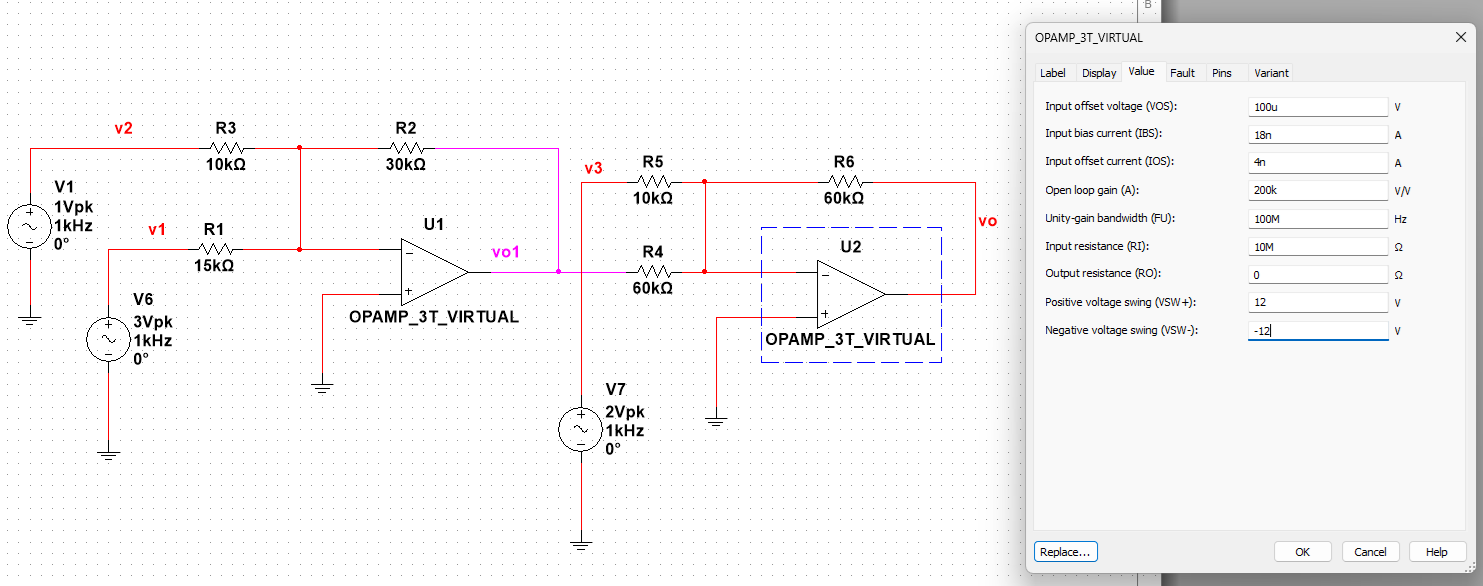
\includegraphics[width=.9\linewidth]{./my-chapters/my-images/Question1/b_machmophong_nonideal.png}
		\caption{Thiết kế mạch $V_{o} = 2V_{1} + 3V_{2} - 6V_{3}$ với OPAMP không lý tưởng.}
	\end{figure}
	
	\begin{figure}[H]
		\centering
		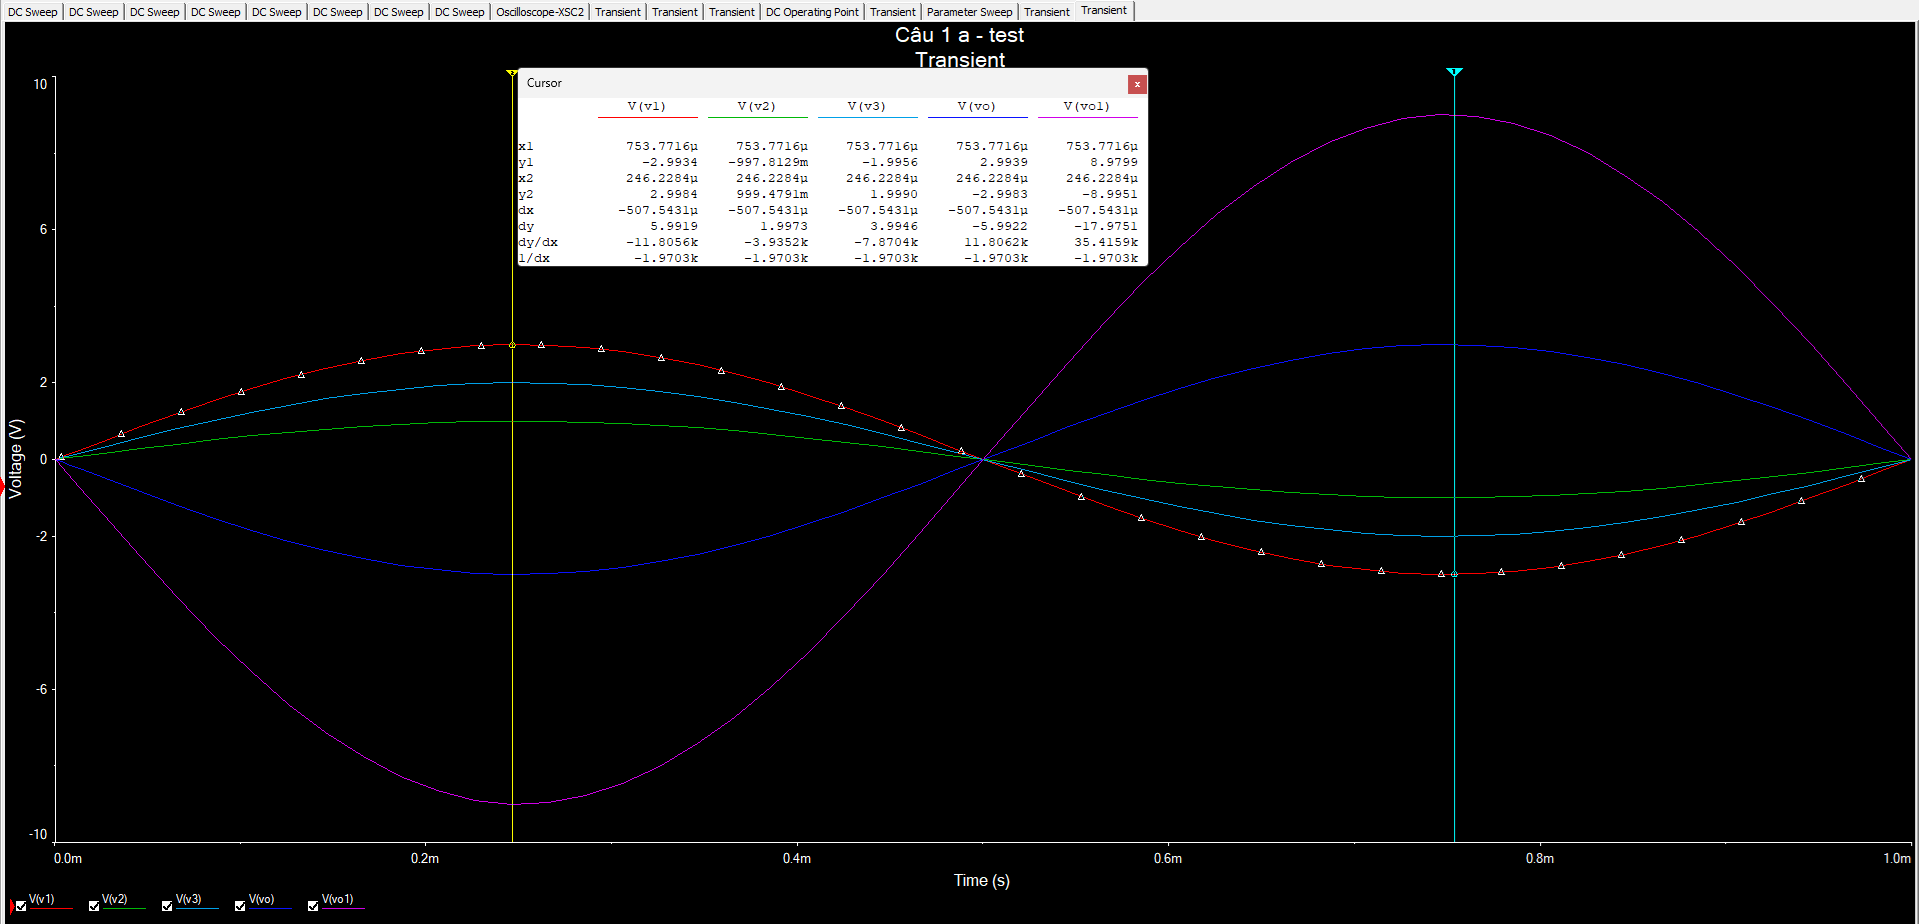
\includegraphics[width=.9\linewidth]{./my-chapters/my-images/Question1/b_ketqua_nonideal.png}
		\caption{Kế quả của mạch $V_{o} = 2V_{1} + 3V_{2} - 6V_{3}$ với OPAMP không lý tưởng.}
	\end{figure}
	
	\begin{minipage}{.7\linewidth}
		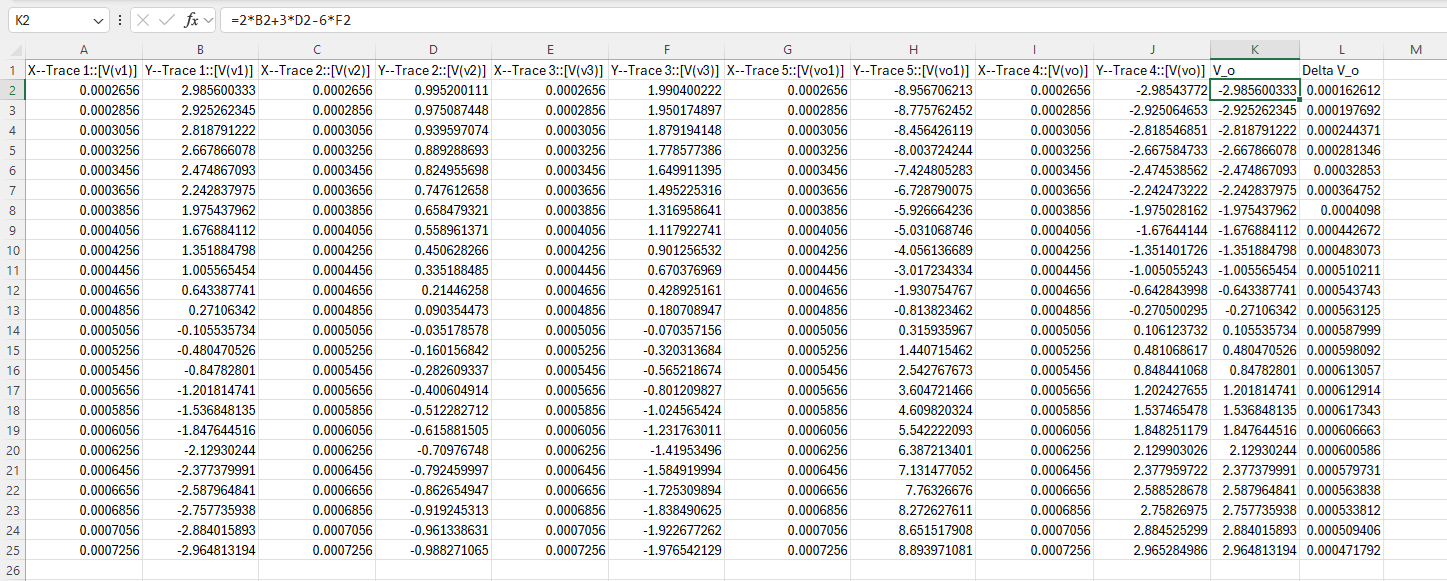
\includegraphics[width=\linewidth]{./my-chapters/my-images/Question1/a_saiso_nonideal.png}
	\end{minipage}
	\begin{minipage}{.3\linewidth}
		\begin{itemize}[label=-]
			\item \finalresult{\Delta V_{o_{max}} = 0.000617343 \,\textsf{V}}
			\item \finalresult{\Delta V_{o_{min}} = 0.000162612 \,\textsf{V}}
		\end{itemize}
	\end{minipage}
\end{itemize}